% =====================================================================
% Artigo LADC 2026 Student Forum — versão em PORTUGUÊS
% Formato: Springer LNCS (llncs.cls)
% Escopo: medição empírica de dependabilidade (SEM modelagem SPN)
%
% COMPILAÇÃO: requer llncs.cls (baixe em
%   https://www.springer.com/gp/computer-science/lncs/conference-proceedings-guidelines)
%   pdflatex artigo_pt.tex  (2x para referências)
% =====================================================================
\documentclass[runningheads]{llncs}

\usepackage[T1]{fontenc}
\usepackage[utf8]{inputenc}
\usepackage{graphicx}
\usepackage{booktabs}
\usepackage{amsmath}
\usepackage{url}
\usepackage{float}
\usepackage[table]{xcolor}
\usepackage[portuguese]{babel}
\AtBeginDocument{\renewcommand{\andname}{e}}
% DOI quebrável em fonte romana (o \doi do llncs é inquebrável e estica linhas)
\AtBeginDocument{\def\doi#1{{\urlstyle{rm}\url{https://doi.org/#1}}}}
\def\UrlBreaks{\do\/\do\-\do\.\do\_}
% --- ajuste de espacamento para o limite de 11 paginas do LADC ---
\usepackage{enumitem}
\setlist{nosep,topsep=2pt,leftmargin=*}
\setlength{\textfloatsep}{10pt plus 2pt minus 2pt}
\setlength{\floatsep}{8pt plus 2pt minus 2pt}
\setlength{\intextsep}{10pt plus 2pt minus 2pt}
\setlength{\abovecaptionskip}{6pt}
\setlength{\belowcaptionskip}{0pt}

\begin{document}

\title{Medição Empírica de Dependabilidade do Apache Cassandra sob
Injeção de Faltas: o Impacto dos Níveis de Consistência}
\titlerunning{Dependabilidade do Cassandra sob Injeção de Faltas}

% Se o forum for double-blind, comente os autores na submissão.
\author{Caio Farias Cavalcanti\inst{1} \and
Gustavo Rau de Almeida Callou\inst{1}}
\authorrunning{C. F. Cavalcanti e G. R. A. Callou}
\institute{Universidade Federal Rural de Pernambuco (UFRPE), Recife--PE, Brasil\\
\email{\{caio.farias,gustavo.callou\}@ufrpe.br}}

\maketitle

\begin{abstract}
Sistemas de banco de dados distribuídos como o Apache Cassandra oferecem níveis
de consistência ajustáveis que regulam o compromisso entre disponibilidade e
consistência. Embora bem compreendido em teoria, esse compromisso carece de
medições empíricas sobre como diferentes níveis de consistência afetam a
dependabilidade do serviço sob faltas reais. Este trabalho apresenta um estudo
de medição que injeta cinco tipos de falta (crash de réplica, crash de
coordenador, atraso de rede, perda de pacotes e partição de rede) no Cassandra sob
três níveis de consistência (ONE, QUORUM, ALL) e três níveis de carga, com três
repetições cada (135 execuções). Os resultados
quantificam dois fenômenos distintos: faltas que geram indisponibilidade (crash
e partição), em que ONE e QUORUM mascaram completamente a falta enquanto ALL
apresenta taxa de erro de até 25\%; e faltas de temporização (atraso e perda),
em que a vazão degrada $\sim$98\% independentemente do nível de consistência.
Mede-se ainda o tempo de reparo (MTTR) por tipo de falta, de $\sim$15\,s (crash)
a $\sim$32\,s (partição). As medições estendem trabalhos anteriores ao
introduzir cenários de partição não estudados previamente e ao fornecer valores
empíricos de disponibilidade observada de serviço e MTTR.

\keywords{Dependabilidade \and Apache Cassandra \and Injeção de faltas \and
Níveis de consistência \and Disponibilidade \and Tolerância a faltas.}
\end{abstract}

% =====================================================================
\section{Introdução}
% Alvo: ~1,5 página
% =====================================================================

Bancos de dados NoSQL distribuídos tornaram-se infraestrutura central de
aplicações de larga escala, oferecendo escalabilidade horizontal e tolerância a
faltas por meio de replicação e consenso. O Apache Cassandra é um representante
notável dessa categoria, adotado por organizações que demandam alta
disponibilidade sobre grandes volumes de dados~\cite{lakshman2010cassandra}. Uma
característica definidora do Cassandra é a \emph{consistência ajustável}: para
cada operação, a aplicação escolhe quantas réplicas devem participar, regulando
explicitamente o compromisso entre consistência e disponibilidade previsto pelo
teorema CAP~\cite{brewer2000cap,gilbert2002cap}.

Esse compromisso é bem compreendido em nível teórico. O que permanece menos
explorado é a \emph{quantificação empírica} de como a escolha do nível de
consistência afeta a dependabilidade do serviço entregue ao cliente quando o
sistema enfrenta faltas reais. Saber que ALL "prioriza consistência" não informa
\emph{quanto} da disponibilidade se perde sob uma falha concreta, nem \emph{quão
rápido} o serviço se recupera. São medidas de
dependabilidade~\cite{avizienis2004basic,meyer1980} de que operadores precisam
para decidir configurações.

Este trabalho aborda essa lacuna por meio de um estudo de medição controlado: um
cluster Cassandra de cinco nós em nuvem é submetido a cinco classes de falta sob
três níveis de consistência e três cargas, registrando-se vazão, latência e taxa
de erro antes, durante e após cada falta.

O objeto de estudo é o nível de consistência, e o Cassandra se presta a isolá-lo
porque o nível é escolhido por operação: ONE, QUORUM e ALL podem ser comparados
no \emph{mesmo} cluster, com os mesmos dados e a mesma falta. Em sistemas
baseados em consenso, como o etcd (Raft), a garantia é em grande parte fixada
pelo protocolo. O método de injeção (\texttt{systemctl}, \texttt{tc/netem},
\texttt{iptables} e série temporal no cliente) não depende do Cassandra; se os
compromissos observados se generalizam fica como trabalho futuro.

As contribuições são: (i) uma metodologia reproduzível de injeção de faltas para
Cassandra, cobrindo crash, temporização, omissão e partição com controle preciso
da linha do tempo, com \emph{scripts} e dados publicamente
disponíveis~\cite{artifact}; (ii) a quantificação empírica do impacto do nível de
consistência sobre a dependabilidade, distinguindo faltas de disponibilidade de
faltas de temporização; e (iii) valores medidos de disponibilidade observada e
MTTR, incluindo cenários de partição não tratados na literatura correlata. O
escopo é restrito à medição: esta é a etapa experimental de um projeto de
graduação, tendo a modelagem analítica como etapa subsequente.

O estudo é guiado por três questões de pesquisa:
\begin{itemize}
\item \textbf{RQ1:} Como o nível de consistência do Cassandra afeta a
disponibilidade do serviço sob faltas de \emph{crash} e partição de rede?
\item \textbf{RQ2:} Como o nível de consistência afeta a degradação de
desempenho sob faltas de temporização de rede (atraso e perda de pacotes)?
\item \textbf{RQ3:} Como diferentes tipos de falta afetam o tempo de
recuperação do Cassandra (MTTR)?
\end{itemize}

A Seção~\ref{sec:related} revisa os trabalhos relacionados e a
Seção~\ref{sec:background}, os conceitos utilizados. A
Seção~\ref{sec:methodology} descreve o desenho experimental e a
Seção~\ref{sec:environment}, o aparato. A Seção~\ref{sec:casestudy} apresenta e
discute os resultados, e a Seção~\ref{sec:conclusion} conclui.

% =====================================================================
\section{Trabalhos Relacionados}
\label{sec:related}
% Alvo: ~1,5 página
% =====================================================================

A avaliação de dependabilidade do Cassandra tem sido abordada por medição e por
modelagem analítica. Ferreira et al.~\cite{ferreira2021} avaliaram
experimentalmente o desempenho do Cassandra sob diferentes níveis de consistência
e cargas, estabelecendo uma base de comparação de vazão e latência em operação
normal, sem caracterizar o comportamento sob indisponibilidade de nós ou
degradação de rede. Adotamos parâmetros de carga compatíveis e acrescentamos uma
fase sistemática de injeção de faltas.

Outros estudos cobrem dimensões complementares. Rosselli et
al.~\cite{rosselli2016} avaliaram a disponibilidade e a tolerância a faltas do
Cassandra medindo o impacto da queda de um nó sobre vazão e latência, sem porém
variar sistematicamente o nível de consistência nem cobrir faltas de rede como
atraso, perda e partição. Rahman et al.~\cite{rahman2012} propuseram um
arcabouço, integrado ao YCSB, para medir anomalias de consistência em sistemas
chave-valor, e o projeto Jepsen~\cite{jepsen} submete bancos distribuídos,
incluindo o Cassandra, a partições e crashes para verificar \emph{violações de
correção}; nosso trabalho, em vez disso, quantifica medidas de dependabilidade
(taxa de erro, degradação de vazão e MTTR) em função do nível de consistência.

Gomes et al.~\cite{gomes2019} propuseram um modelo analítico de dependabilidade
para o Cassandra baseado em redes de Petri estocásticas generalizadas (GSPN),
estimando disponibilidade a partir de MTTF e MTTR adotados de forma hipotética
(MTTF de 2880\,h e 5760\,h; MTTR de 0,5\,h e 1\,h), à falta de medições diretas;
este trabalho fornece MTTR \emph{medido empiricamente} por tipo de falta.

A injeção de faltas é técnica consolidada de \emph{fault forecasting} para a
avaliação experimental de
dependabilidade~\cite{avizienis2004basic,borges2025,silva2025models}. Partições
de rede, que materializam o teorema CAP, não foram, até onde sabemos,
caracterizadas como medida de dependabilidade nos trabalhos correlatos sobre
Cassandra.

% =====================================================================
\section{Fundamentação Teórica}
\label{sec:background}
% Alvo: ~2,0 páginas
% =====================================================================

\subsection{Dependabilidade e a cadeia falta--erro--falha}

Dependabilidade é a capacidade de um sistema de entregar um serviço no qual se
pode justificadamente confiar~\cite{avizienis2004basic}, englobando atributos
como disponibilidade (prontidão para o serviço correto), confiabilidade
(continuidade do serviço correto) e manutenibilidade (capacidade de reparo). O
arcabouço de Avizienis et al. estrutura as ameaças à dependabilidade na cadeia
causal \emph{falta $\rightarrow$ erro $\rightarrow$ falha}: uma \textbf{falta} é a
causa hipotética ou real de um erro (p.\,ex., um processo que termina); um
\textbf{erro} é a parte do estado do sistema que pode levar a uma falha (p.\,ex., uma
réplica inalcançável); e uma \textbf{falha} ocorre quando o serviço entregue
desvia do correto (p.\,ex., uma operação que retorna erro ao cliente). Entre o erro e a falha atuam os \emph{mecanismos de tolerância a
faltas}: quando um mecanismo impede que um erro se propague até o serviço,
diz-se que a falta foi \emph{mascarada}; a injeção controlada de faltas mede se
cada falta atravessa essas defesas.

\subsection{Replicação e níveis de consistência do Cassandra}

O Cassandra particiona os dados em um anel de \emph{tokens} e replica cada
partição em um número de nós dado pelo \emph{fator de replicação} ($RF$). Com $RF=3$, cada item existe em três nós distintos, o que
constitui seu mecanismo fundamental de tolerância a faltas.

O \emph{nível de consistência} (Consistency Level, CL) determina, por operação,
quantas réplicas devem responder para que ela seja considerada bem-sucedida:
\textbf{ONE} exige uma réplica (tolera a perda de até $RF-1$ réplicas); \textbf{QUORUM} exige a maioria, $\lfloor RF/2 \rfloor + 1$
réplicas (duas, para $RF=3$; tolera a perda de uma); e \textbf{ALL} exige todas
as $RF$ réplicas (não tolera perda alguma).

Um nível de consistência é um parâmetro por operação, e não um \emph{modelo} de
consistência; o modelo resultante depende dos níveis usados nas leituras ($R$
réplicas) e nas escritas ($W$). Com ONE, uma leitura pode retornar dado
desatualizado, e o sistema oferece apenas \emph{consistência eventual}. Quando
$R+W>RF$, como com QUORUM em ambas ou com ALL, todo conjunto de leitura
intersecta as réplicas que confirmaram a última escrita concluída. Isso ainda é
mais fraco que a \emph{linearizabilidade}, que no Cassandra exige
\emph{lightweight transactions} (Paxos), não usadas aqui. Medimos o
\emph{custo} em disponibilidade e desempenho de cada nível, e não a consistência
obtida, objeto de~\cite{rahman2012,jepsen}.

O CL é, portanto, um mecanismo em nível de aplicação para controlar o
comportamento observado durante falhas de nó e de rede: ONE favorece
disponibilidade (responde com qualquer réplica alcançável), enquanto ALL
recusa-se a responder sem todas. Um aspecto importante para
interpretar os resultados é que, em Cassandra, \emph{toda escrita é enviada a
todas as réplicas} independentemente do CL, que define apenas quantas
confirmações o coordenador aguarda.

\subsection{Atributos de dependabilidade mensuráveis}

A partir da observação do serviço sob faltas derivam-se as medidas de interesse,
provenientes de duas tradições complementares: os atributos da taxonomia de
Avizienis et al.~\cite{avizienis2004basic} e a \emph{performability} de
Meyer~\cite{meyer1980}. A \textbf{disponibilidade} (prontidão para o serviço
correto) é medida no nível operacional, pela fração de operações atendidas
corretamente, isto é, $A = 1 - (\text{erros}/\text{total de operações})$;
chamamos essa grandeza de \emph{disponibilidade observada de serviço}. Ela se
afasta da disponibilidade estacionária clássica
$A = \text{MTTF}/(\text{MTTF}+\text{MTTR})$ por duas razões: as faltas são
injetadas em instantes fixos, de modo que não há MTTF a medir; e, num sistema que
atende requisições, cada operação é uma demanda de serviço, de modo que a fração
atendida corretamente é a disponibilidade que o cliente experimenta, a forma
baseada em requisições usada em objetivos de nível de serviço. Como depende do
intervalo de observação, reportamo-la sobre a execução inteira e dentro da
janela de falta. A
\textbf{performability}~\cite{meyer1980} é o grau de degradação de vazão e
latência durante a falta, quando o serviço permanece disponível mas com qualidade
reduzida; não é um atributo da taxonomia de Avizienis et al., e sim uma medida
composta de desempenho e dependabilidade, adequada a sistemas degradáveis. A
\textbf{manutenibilidade} é avaliada pelo tempo de recuperação (MTTR) após a
falta injetada.

% =====================================================================
\section{Metodologia}
\label{sec:methodology}
% Alvo: ~1,5 página
% =====================================================================

\subsection{Desenho experimental}

O estudo organiza-se em duas fases. A \emph{fase de baseline} mede vazão e
latência em regime normal, variando o nível de consistência (ONE, QUORUM, ALL) e
a carga (10, 30 e 50 \emph{threads} de cliente), com três repetições por célula.
A \emph{fase de injeção de faltas} acrescenta a dimensão do tipo de falta,
totalizando $5 \times 3 \times 3 \times 3 = 135$ execuções controladas.

\subsection{Tipos de falta injetados}

Cinco tipos de falta cobrem as principais classes da taxonomia de
dependabilidade. \textbf{Crash de réplica} (\texttt{node\_crash}): término do
processo Cassandra em um nó réplica, via \texttt{systemctl stop}, que testa o
mascaramento por replicação. Trata-se de um desligamento \emph{ordenado}, em que
o nó anuncia sua saída aos pares; a escolha isola a perda da réplica do atraso de
detecção de falha e permite reinício limpo numa bateria automatizada longa (o
término abrupto é discutido nas ameaças à validade). \textbf{Crash de coordenador}
(\texttt{coord\_crash}): término do processo no nó de contato do cliente, testando
o \emph{failover} de roteamento do \emph{driver}. \textbf{Atraso de rede} (\texttt{net\_delay}): inserção de
$200\,\text{ms} \pm 50\,\text{ms}$ de latência no tráfego de saída de um nó, via
\texttt{tc/netem} (falta de temporização). \textbf{Perda de pacotes}
(\texttt{net\_loss}): descarte de 25\% dos pacotes de saída de um nó, também via
\texttt{tc/netem} (falta de omissão). \textbf{Partição de rede}
(\texttt{net\_partition}): isolamento de um nó em relação aos demais, via regras
\texttt{iptables}, mantendo o nó vivo porém incomunicável, o que materializa o
cenário do teorema CAP.

\subsection{Linha do tempo de cada execução}

Cada execução dura 300\,s e segue uma linha do tempo controlada
(Fig.~\ref{fig:timeline}): 60\,s em regime saudável; injeção da falta em
$t=60\,$s; falta ativa por 90\,s; remoção em $t=150\,$s; e recuperação até
$t=300\,$s. A janela de 90\,s excede o tempo de detecção de falha do protocolo de
\emph{gossip} do Cassandra (da ordem de 10\,s), garantindo uma janela de falta
efetivamente detectada e longa o bastante para medição.

% ---- PLACEHOLDER FIGURA 1 ----
\begin{figure}[t]
\centering
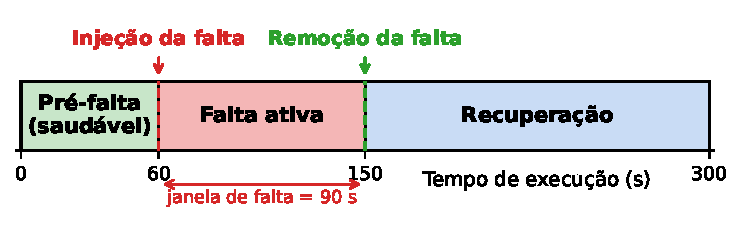
\includegraphics[width=0.75\textwidth]{figs/fig_timeline_pt.pdf}
\caption{Linha do tempo controlada de uma execução de injeção de faltas.}
\label{fig:timeline}
\end{figure}

\subsection{Carga de trabalho e métricas}

A carga é gerada pelo YCSB (Yahoo! Cloud Serving Benchmark)~\cite{ycsb} com o
\emph{Workload~A} (50\% leituras, 50\% atualizações) sobre 100.000 registros,
com execuções limitadas por tempo (300\,s). O YCSB registra a cada 10\,s a
vazão, a latência e as contagens de operações bem-sucedidas e com erro; os
instantes reais de injeção, remoção e recuperação, registrados pelo injetor,
alinham essa série às janelas pré, durante e pós-falta.

Dessas séries calculamos a \textbf{taxa de erro} (erros sobre total de operações)
e a \textbf{disponibilidade observada de serviço} ($1-$ taxa de erro), usadas
para crash e partição; a \textbf{degradação de vazão},
$1 - \text{vazão}_{\text{durante}}/\text{vazão}_{\text{pré}}$, usada para atraso e
perda; e o \textbf{MTTR}, o intervalo entre a remoção da falta e a confirmação, via
\texttt{nodetool status}, de que o cluster voltou a cinco nós ativos. Por
construção, o MTTR só é significativo para faltas que derrubam o nó do
\emph{gossip} (crash e partição); para faltas de temporização, a recuperação
relevante é a da vazão, observável na janela pós-falta.

% =====================================================================
\section{Ambiente e Aparato Experimental}
\label{sec:environment}
% Alvo: ~1,5 página
% =====================================================================

\subsection{Infraestrutura}


O experimento foi executado no Google Cloud Platform, na zona
\texttt{us-central1-a} (Fig.~\ref{fig:arquitetura}). O cluster Cassandra
tem cinco máquinas virtuais \texttt{e2-standard-2} (2 vCPUs, 8\,GB de
RAM cada) executando Cassandra~4.1 sobre Ubuntu~22.04, e a carga é gerada por uma
VM dedicada (\texttt{e2-medium}, 2 vCPUs, 4\,GB) co-localizada na mesma zona, de
modo que a latência cliente--cluster ($\sim$0,3\,ms) não seja fator de confusão.

\begin{figure}[t]
\centering
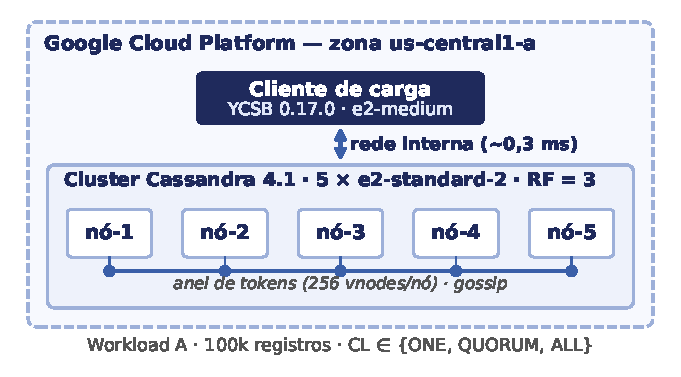
\includegraphics[width=0.72\textwidth]{figs/arch_pt.pdf}
\caption{Arquitetura do ambiente experimental: cluster Cassandra~4.1 de cinco
nós \texttt{e2-standard-2} (RF=3, \texttt{SimpleStrategy}) e cliente de carga
YCSB (\texttt{e2-medium}), co-localizados na zona \texttt{us-central1-a} do
Google Cloud Platform.}
\label{fig:arquitetura}
\end{figure}

\subsection{Configuração do Cassandra}
\label{sec:cassandra-config}

O cluster usa $RF=3$ com \texttt{SimpleStrategy} (adequada a um único
\emph{datacenter}), \texttt{num\_tokens}=256, \texttt{Murmur3\-Partitioner},
\emph{snitch} \texttt{Gossiping\-Property\-File\-Snitch} e dois nós \emph{seeds}. A
distribuição de \emph{tokens} resultante atribui a cada nó $\sim$58--62\% do
espaço de chaves em propriedade efetiva, o que é relevante para a interpretação
dos resultados sob CL=ALL.

\subsection{Carga e ferramentas}

A geração de carga utiliza o YCSB~0.17.0~\cite{ycsb}. A injeção de faltas é
realizada por \emph{scripts} que orquestram, sincronizados com a execução do
YCSB, o término e o reinício de processos (\texttt{systemctl}) para os crashes, a
manipulação de disciplina de fila (\texttt{tc/netem}) para atraso e perda, e
regras de \emph{firewall} (\texttt{iptables}) para a partição. Verificação
pós-remoção e limpeza idempotente impedem que estado residual de falta contamine
execuções subsequentes, requisito crítico em uma bateria longa de execuções
automatizadas. A Tabela~\ref{tab:params} resume os parâmetros centrais. Os
\emph{scripts} de injeção e de análise, os logs brutos e os dados por execução
estão publicamente disponíveis~\cite{artifact}.

\begin{table}[t]
\centering
\scriptsize
\renewcommand{\arraystretch}{1.15}
\setlength{\tabcolsep}{3.5pt}
\caption{Parâmetros do experimento.}
\label{tab:params}
\begin{tabular}{llll}
\toprule
\textbf{Parâmetro} & \textbf{Valor} & \textbf{Parâmetro} & \textbf{Valor} \\
\midrule
\rowcolor{gray!12}
Nós Cassandra & 5 $\times$ e2-standard-2 & Carga (threads) & 10, 30, 50 \\
Cliente de carga & 1 $\times$ e2-medium & Repetições/célula & 3 \\
\rowcolor{gray!12}
Versão do Cassandra & 4.1 & Carga de trabalho & YCSB A (50/50 leit./atual.) \\
Fator de replicação & 3 (SimpleStrategy) & Registros & 100.000 \\
\rowcolor{gray!12}
Níveis de consistência & ONE, QUORUM, ALL & Duração & 300\,s \\
Execuções (faltas) & 135 & Janela de falta & 90\,s ($t=60$--150\,s) \\
\bottomrule
\end{tabular}
\end{table}

% =====================================================================
\section{Estudo de Caso: Resultados e Discussão}
\label{sec:casestudy}
% Alvo: ~2,0 páginas
% =====================================================================

Na fase de \emph{baseline} sem faltas, o coeficiente de variação entre
repetições ficou abaixo de 3\%. Os resultados agrupam-se pelo atributo
predominante: disponibilidade (crash, partição) e \emph{performability} (faltas
de temporização).

\subsection{Disponibilidade sob crash e partição}

A Tabela~\ref{tab:availability} apresenta a taxa de erro média por tipo de falta
e nível de consistência. O padrão é nítido e consistente com a teoria do quórum:
sob crash de réplica ou de coordenador, ONE e QUORUM mantêm taxa de erro
praticamente nula (zero operações com falha em todas as células, exceto uma
única em $2{,}6\times10^{7}$ sob ONE no crash de coordenador), pois com $RF=3$ a
perda de uma réplica deixa duas disponíveis, suficientes para ONE (uma) e QUORUM
(duas). A falta é, portanto, \emph{mascarada} pela replicação, e ambos
entregam disponibilidade observada de serviço de $\sim$100\%. Sob ALL, a
exigência das três réplicas faz falhar toda operação cujo conjunto de réplicas
inclua o nó indisponível, resultando em taxa de erro média de $\sim$24--25\%
sobre a execução completa, valor menor que a fração de réplicas afetadas
porque é diluído pelos períodos saudáveis.

A diluição não é proporcional ao tempo (90 de 300\,s, 30\%). A vazão após a
falta ($\sim$4400--5700\,ops/s) é menor que antes dela ($\sim$7100--8200\,ops/s),
de modo que a janela de falta concentra 33--41\% das operações da execução.
Atribuímos a vazão pós-falta menor à reintegração do nó, que sob ALL participa de
toda operação sobre suas réplicas; essa explicação é inferida do comportamento do
Cassandra, e não instrumentada.

Medida \emph{dentro da janela de falta}, a partir das amostras de 10\,s do YCSB,
a taxa de erro sob ALL é de 56,7\% no crash de réplica, 55,6\% no de coordenador
e 56,7\% na partição (desvio padrão inferior a 0,1 ponto). Crash de réplica e
partição incidem sobre o \emph{mesmo} nó e coincidem na terceira casa (56,65\% e
56,66\%): o tipo de falta altera por quanto tempo as operações falham, e não
quais. Os três ficam próximos dos 60\% esperados de $RF=3$ sobre cinco nós sob
acesso uniforme; atribuímos a diferença à distribuição \emph{zipfian} do
\emph{Workload~A}~\cite{ycsb}. Parte dos erros ocorre \emph{após} a remoção: o
serviço retorna $\sim$13--15\,s após a remoção de um crash e $\sim$3\,s após a
remoção da partição. A taxa média (Tabela~\ref{tab:availability}) e a
instantânea são complementares: a primeira quantifica o custo amortizado ao longo
da execução, e a segunda isola a severidade percebida enquanto o nó está
indisponível.

\begin{table}[t]
\centering
\caption{Taxa de erro (\%) por tipo de falta e nível de consistência (média
$\pm$ desvio padrão sobre cargas e repetições; $n=9$ por célula: 3 cargas
$\times$ 3 repetições). Entre parênteses, o número absoluto de operações com falha
somado sobre as nove execuções; cada célula totaliza
$1{,}6$--$2{,}8\times10^{7}$ operações.}
\label{tab:availability}
\small
\setlength{\tabcolsep}{2pt}
\begin{tabular}{lccc}
\toprule
\textbf{Tipo de falta} & \textbf{ONE} & \textbf{QUORUM} & \textbf{ALL} \\
\midrule
Crash de réplica      & 0,00$\pm$0,00 (0) & 0,00$\pm$0,00 (0) & 24,29$\pm$4,24 (3.902.961) \\
Crash de coordenador  & 0,00$\pm$0,00 (1) & 0,00$\pm$0,00 (0) & 25,25$\pm$1,45 (4.008.616) \\
Partição de rede      & 0,05$\pm$0,05 (16.305) & 0,05$\pm$0,10 (9.768) & 19,01$\pm$1,74 (3.442.518) \\
\bottomrule
\end{tabular}
\end{table}

Um resultado original está na comparação entre crash e partição sob ALL: a
partição produz taxa de erro média \emph{menor} ($\sim$19\%) que o crash
($\sim$24--25\%), embora a severidade instantânea medida no \emph{mesmo} nó alvo
seja idêntica ($\sim$56,7\%). A diferença não está, portanto, no que ocorre
\emph{durante} a falta, pois sob ALL um nó isolado porém vivo é tão inalcançável
quanto um nó morto, e sim na
\emph{duração} do comprometimento do serviço: $\sim$98\,s na partição contra
$\sim$124--129\,s nos crashes. Remover uma regra \texttt{iptables} restaura a
conectividade de imediato, ao passo que um processo reiniciado precisa antes
reingressar no \emph{cluster}. Essa dissociação entre \emph{remoção da falta} e
\emph{restauração do serviço} não havia sido caracterizada em trabalhos
correlatos. A Figura~\ref{fig:panel} (centro) mostra ainda um breve pico de erro
de QUORUM ($\sim$18\%) nos primeiros $\sim$10\,s da partição, invisível nas
métricas agregadas, que atribuímos à convergência do \emph{gossip}.

% ---- FIGURA 3: painel das 3 falhas-chave ----
\begin{figure}[t]
\centering
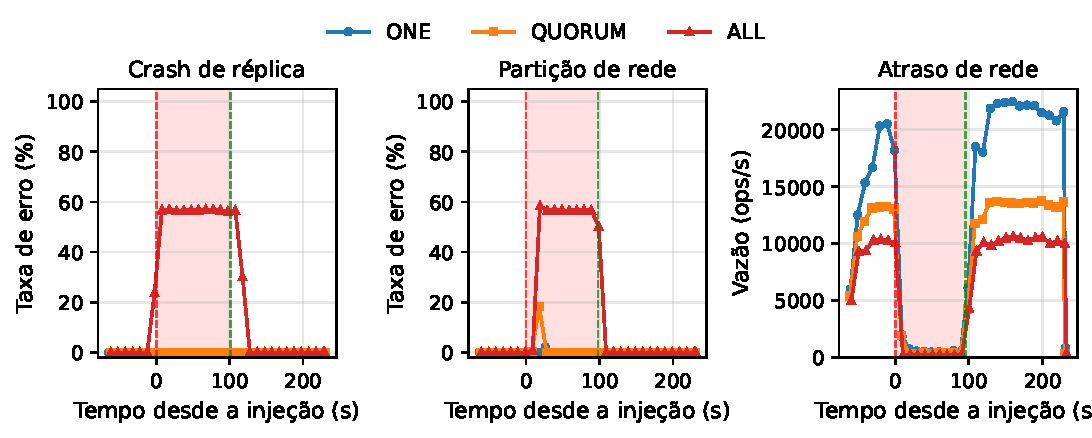
\includegraphics[width=\textwidth]{figs/panel_3faults_pt.pdf}
\caption{Séries temporais a 50 \emph{threads} (repetição mediana), com o tempo
realinhado à injeção da falta ($t=0$) e a janela de falta sombreada. Esquerda e
centro: taxa de erro sob crash de réplica e partição: apenas ALL reage, com
ONE e QUORUM em $\sim$0\%. Direita: vazão sob atraso de rede, os três níveis
degradam conjuntamente.}
\label{fig:panel}
\end{figure}

\subsection{Recuperabilidade: tempo de reparo}

A Tabela~\ref{tab:mttr} apresenta o MTTR por tipo de falta (RQ3). Os crashes se
recuperam em $\sim$15--19\,s e a partição em $\sim$32\,s, o que atribuímos à
reconvergência das visões do \emph{gossip} dos dois lados. Esse MTTR de plano de
controle difere da recuperação percebida pelo cliente: na partição o serviço
retorna $\sim$3\,s após a remoção, muito antes de o \emph{gossip} convergir,
enquanto nos crashes as duas grandezas praticamente coincidem ($\sim$13--15\,s).
Modelos parametrizados por MTTR devem explicitar qual recuperação representa a
indisponibilidade.

\begin{table}[t]
\centering
\caption{Tempo de reparo (s): da remoção da falta até \texttt{nodetool status}
mostrar cinco nós ativos (plano de controle). Média $\pm$ desvio padrão; $n=27$
por tipo de falta (3 níveis $\times$ 3 cargas $\times$ 3 repetições).}
\label{tab:mttr}
\small
\setlength{\tabcolsep}{5pt}
\begin{tabular}{lccc}
\toprule
\textbf{Tipo de falta} & \textbf{Média $\pm$ DP} & \textbf{Mín.} & \textbf{Máx.} \\
\midrule
Crash de réplica     & 15,19$\pm$2,76 & 11 & 25 \\
Crash de coordenador & 19,15$\pm$7,27 & 12 & 34 \\
Partição de rede     & 31,93$\pm$7,90 & 23 & 47 \\
\bottomrule
\end{tabular}
\end{table}

\subsection{Performability sob atraso e perda}

A Tabela~\ref{tab:performability} apresenta a degradação de vazão sob faltas de
temporização. A degradação é severa ($\sim$97--98\%) e \emph{praticamente
independente do nível de consistência}: as diferenças entre níveis são da ordem
do desvio padrão (0,2--0,6 ponto). A taxa de erro permanece nula, tratando-se de
falha de temporização, e não de omissão. Atribuímos a independência do CL ao
caminho de escrita: toda escrita é enviada a todas as réplicas, de modo que um nó
lento atrasa as operações que o envolvem, qualquer que seja o número de
confirmações aguardadas.

O p99 da execução inteira (9--22\,ms) esconde isso, pois as operações lentas são
$\sim$1\% do total. Por janela de 10\,s, o p99 sobe de $\sim$11\,ms para uma
mediana de $\sim$920\,ms durante a falta, e a perda é pior que o atraso
($\sim$1,2--2,3\,s contra $\sim$0,6--0,9\,s) apesar de degradação de vazão
igual.

\begin{table}[t]
\centering
\caption{Degradação de vazão (\%) sob faltas de temporização (média $\pm$ desvio
padrão sobre cargas e repetições; $n=9$ por célula).}
\label{tab:performability}
\small
\setlength{\tabcolsep}{5pt}
\begin{tabular}{lccc}
\toprule
\textbf{Tipo de falta} & \textbf{ONE} & \textbf{QUORUM} & \textbf{ALL} \\
\midrule
Atraso de rede   & 97,54$\pm$0,45 & 97,60$\pm$0,44 & 98,35$\pm$0,61 \\
Perda de pacotes & 97,22$\pm$0,53 & 96,70$\pm$0,22 & 98,28$\pm$0,28 \\
\bottomrule
\end{tabular}
\end{table}

\subsection{Síntese}

O nível de consistência controla o compromisso \emph{sob faltas de
disponibilidade} (RQ1), mas é \emph{inócuo sob faltas de temporização} (RQ2):
protege contra um nó indisponível, não contra degradação de rede.

\subsection{Ameaças à validade}

Seis ameaças devem ser registradas. A primeira é de generalização: cada tipo de
falta foi injetado em um \emph{único nó alvo} fixo, escolha deliberada que
isola o tipo de falta como único fator variável entre crash e partição, mas torna
a severidade absoluta de $\sim$56,7\% específica da faixa de \emph{tokens} daquele
nó e das chaves quentes do gerador \emph{zipfian}. Dessa mesma dependência decorre
a variância mais alta observada sob ALL em carga elevada. Segundo, três
repetições por configuração ($n=9$ por falta e nível, $n=27$ por falta no MTTR)
tornam as estimativas de dispersão imprecisas; as conclusões apoiam-se em
contrastes muito maiores (zero contra 19--25\% de erros; 97--98\% de degradação
em todos os níveis), e diferenças da ordem de um desvio padrão não são
afirmadas. O
MTTR é sondado via SSH, o que limita sua resolução a $\sim$10\,s. Terceiro, os
crashes são desligamentos ordenados. Uma verificação posterior em um novo cluster
(30 \emph{threads}, quatro repetições) encontrou zero operações com falha sob ONE
e QUORUM também com \texttt{SIGKILL} e com queda de máquina emulada; mas sob ALL
o serviço levou $\sim$48\,s para retornar após \texttt{SIGKILL} (contra
$\sim$18\,s após parada ordenada), e a queda de máquina causou $\sim$20\,s em
que mais de 1\% das operações levaram mais de 200\,ms sob ONE e QUORUM. Nossos
tempos de recuperação de crash são, portanto, limites inferiores para falhas
abruptas. Quarto, a injeção em instante fixo não mede o MTTF, apenas o MTTR.
Quinto, o cliente usou os cinco
nós como pontos de contato sob balanceamento padrão; roteamento sensível à
latência poderia atenuar a degradação sob faltas de temporização. Por fim, uma
execução de partição apresentou comportamento anômalo por instabilidade
transitória do cluster, tendo sido reexecutada após verificação de saúde.

% =====================================================================
\section{Conclusão}
\label{sec:conclusion}
% Alvo: ~1,0 página
% =====================================================================

Este trabalho mediu o impacto dos níveis de consistência do Cassandra sobre a
disponibilidade, o desempenho e a recuperação do serviço sob injeção controlada
de faltas. Em 135 execuções, crash e partição são mascarados por ONE e QUORUM,
mas causam $\sim$20--25\% de erro sob ALL, enquanto faltas de temporização
degradam a vazão em $\sim$98\% em todos os níveis. O MTTR vai de $\sim$15\,s
(crash) a $\sim$32\,s (partição), e a restauração do serviço se dissocia da
remoção da falta: $\sim$3\,s após uma partição, mas só depois que o nó que caiu
reingressa.

Este artigo relata a etapa experimental de um projeto de pesquisa de graduação em
andamento. Como trabalho futuro, pretende-se aumentar as repetições por célula;
injetar crashes abruptos e faltas múltiplas, concorrentes ou correlacionadas;
investigar outras cargas e fatores de replicação; aplicar o método a outros
sistemas, como armazenamentos baseados em Raft (p.\,ex., etcd), para testar se
os compromissos se generalizam; e construir um modelo analítico de dependabilidade
(redes de Petri estocásticas ou diagramas de blocos de confiabilidade)
parametrizado pelo MTTR aqui medido, o que permitirá validação cruzada entre
disponibilidades medidas e previstas, além de análise de sensibilidade ao MTTF.

% =====================================================================
\begin{thebibliography}{10}
\setlength{\itemsep}{-1pt plus 0.2pt}

\bibitem{lakshman2010cassandra}
Lakshman, A., Malik, P.: Cassandra: a decentralized structured storage system.
ACM SIGOPS Operating Systems Review \textbf{44}(2), 35--40 (2010)

\bibitem{brewer2000cap}
Brewer, E.A.: Towards robust distributed systems. In: Proc. ACM PODC, pp. 7--10
(2000)

\bibitem{gilbert2002cap}
Gilbert, S., Lynch, N.: Brewer's conjecture and the feasibility of consistent,
available, partition-tolerant web services. ACM SIGACT News \textbf{33}(2),
51--59 (2002)

\bibitem{avizienis2004basic}
Avi\v{z}ienis, A., Laprie, J.C., Randell, B., Landwehr, C.: Basic concepts and
taxonomy of dependable and secure computing. IEEE Trans. Dependable and Secure
Computing \textbf{1}(1), 11--33 (2004)

\bibitem{meyer1980}
Meyer, J.F.: On evaluating the performability of degradable computing systems.
IEEE Trans. Computers \textbf{C-29}(8), 720--731 (1980).
\doi{10.1109/TC.1980.1675654}

\bibitem{ferreira2021}
Ferreira, S., Andrade, E., Mendonça, J.: Uma abordagem experimental para
avaliar os níveis de consistência do banco de dados NoSQL Cassandra. In: Anais
do XXII Simpósio em Sistemas Computacionais de Alto Desempenho (WSCAD),
pp. 156--167. SBC, Porto Alegre (2021). \doi{10.5753/wscad.2021.18520}

\bibitem{borges2025}
Borges, I., Andrade, E., Silva, F.A., Callou, G.: Availability evaluation of a
video surveillance system with distributed storage. Cluster Computing (2025).
\doi{10.1007/s10586-024-04962-x}

\bibitem{silva2025models}
Silva, A., Callou, G.: Models for availability evaluation of file servers in
private clouds. Computing (2025).
\doi{10.1007/s00607-024-01372-0}

\bibitem{gomes2019}
Gomes, C., Borba, E., Tavares, E., Nogueira de O. Junior, M.: Performability
model for assessing NoSQL DBMS consistency. In: Proc. 2019 IEEE International
Systems Conference (SysCon), pp. 1--6. IEEE (2019).
\doi{10.1109/SYSCON.2019.8836757}

\bibitem{rosselli2016}
Rosselli, M., Niemann, R., Ivanov, T., Tolle, K., Zicari, R.V.: Benchmarking the
availability and fault tolerance of Cassandra. In: Big Data Benchmarking (WBDB
2015). LNCS, vol. 10044, pp. 87--95. Springer, Cham (2016).
\doi{10.1007/978-3-319-49748-8_5}

\bibitem{rahman2012}
Rahman, M.R., Golab, W., AuYoung, A., Keeton, K., Wylie, J.J.: Toward a
principled framework for benchmarking consistency. In: Proc. 8th USENIX Workshop
on Hot Topics in System Dependability (HotDep). USENIX Association (2012)

\bibitem{jepsen}
Kingsbury, K.: Jepsen: Cassandra. Relatório de análise Jepsen (2013).
\url{https://aphyr.com/posts/294-jepsen-cassandra}, acesso em 17 set. 2026

\bibitem{ycsb}
Cooper, B.F., Silberstein, A., Tam, E., Ramakrishnan, R., Sears, R.:
Benchmarking cloud serving systems with YCSB. In: Proc. ACM SoCC, pp. 143--154
(2010)

\bibitem{artifact}
Cavalcanti, C.F., Callou, G.R.A.: Fault-injection scripts and data for
``Empirical Dependability Measurement of Apache Cassandra under Fault
Injection'' (2026).
\url{https://github.com/caaiofarias/cassandra-fault-injection-ladc2026}

\end{thebibliography}

\end{document}